\mysection{Trouver les bonnes instructions}

Si le programme utilise des instructions FPU et qu'il n'y en a que quelques une dans
le code, on peut essayer de les vérifier chacunes manuellement avec un débogueur.

\par Par exemple, nous pouvons être intéressés de comprendre comment Microsoft Excel
calcule la formule entrée par l'utilisateur.
Par exemple, l'opération de division.

\myindex{\GrepUsage}
\myindex{x86!\Instructions!FDIV}

Si nous chargeons excel.exe (d'Office 2010) version 14.0.4756.1000 dans \IDA, faisons
un listing complet et cherchons chaque instruction \FDIV (sauf celle qui utilisent
une constante comme second opérande---évidemment, elles ne nous intéressent pas):

\begin{lstlisting}
cat EXCEL.lst | grep fdiv | grep -v dbl_ > EXCEL.fdiv
\end{lstlisting}

\dots nous voyons alors qu'il y en a 144.

\par Nous pouvons entrer une chaîne comme \TT{=(1/3)} dans Excel et vérifier chaque
instruction.

\myindex{tracer}

\par En vérifiant chaque instruction dans un débogueur ou \tracer
(on peut vérifier 4 instructions à la fois),
nous avons de la chance et l'instruction que nous cherchons n'est que la 14ème:

\begin{lstlisting}[style=customasmx86]
.text:3011E919 DC 33          fdiv    qword ptr [ebx]
\end{lstlisting}

\begin{lstlisting}
PID=13944|TID=28744|(0) 0x2f64e919 (Excel.exe!BASE+0x11e919)
EAX=0x02088006 EBX=0x02088018 ECX=0x00000001 EDX=0x00000001
ESI=0x02088000 EDI=0x00544804 EBP=0x0274FA3C ESP=0x0274F9F8
EIP=0x2F64E919
FLAGS=PF IF
FPU ControlWord=IC RC=NEAR PC=64bits PM UM OM ZM DM IM
FPU StatusWord=
FPU ST(0): 1.000000
\end{lstlisting}

\ST{0} contient le premier argument (1) et le second est dans \TT{[EBX]}.\\
\\
\myindex{x86!\Instructions!FDIV}

L'instruction après \FDIV (\TT{FSTP}) écrit le résultat en mémoire:\\

\begin{lstlisting}[style=customasmx86]
.text:3011E91B DD 1E          fstp    qword ptr [esi]
\end{lstlisting}

Si nous mettons un point d'arrêt dessus, nous voyons le résultat:

\begin{lstlisting}
PID=32852|TID=36488|(0) 0x2f40e91b (Excel.exe!BASE+0x11e91b)
EAX=0x00598006 EBX=0x00598018 ECX=0x00000001 EDX=0x00000001
ESI=0x00598000 EDI=0x00294804 EBP=0x026CF93C ESP=0x026CF8F8
EIP=0x2F40E91B
FLAGS=PF IF
FPU ControlWord=IC RC=NEAR PC=64bits PM UM OM ZM DM IM
FPU StatusWord=C1 P
FPU ST(0): 0.333333
\end{lstlisting}

Pour blaguer, nous pouvons modifier le résultat au vol:

\begin{lstlisting}
tracer -l:excel.exe bpx=excel.exe!BASE+0x11E91B,set(st0,666)
\end{lstlisting}

\begin{lstlisting}
PID=36540|TID=24056|(0) 0x2f40e91b (Excel.exe!BASE+0x11e91b)
EAX=0x00680006 EBX=0x00680018 ECX=0x00000001 EDX=0x00000001
ESI=0x00680000 EDI=0x00395404 EBP=0x0290FD9C ESP=0x0290FD58
EIP=0x2F40E91B
FLAGS=PF IF
FPU ControlWord=IC RC=NEAR PC=64bits PM UM OM ZM DM IM
FPU StatusWord=C1 P
FPU ST(0): 0.333333
Set ST0 register to 666.000000
\end{lstlisting}

Excel affiche 666 dans la cellule, achevant de nous convaincre que nous avons trouvé
le bon endroit.

\begin{figure}[H]
\centering
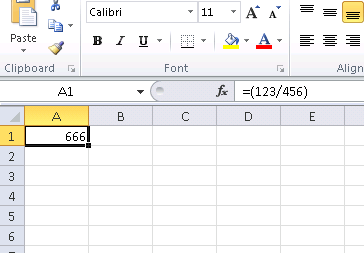
\includegraphics[width=0.6\textwidth]{digging_into_code/Excel_prank.png}
\caption{La blague a fonctionné}
\end{figure}

Si nous essayons la même version d'Excel, mais en x64, nous allons y trouver seulement
12 instructions \FDIV, et celle que nous cherchons est la troisième.

\begin{lstlisting}
tracer.exe -l:excel.exe bpx=excel.exe!BASE+0x1B7FCC,set(st0,666)
\end{lstlisting}

\myindex{x86!\Instructions!DIVSD}

Il semble que le compilateur a remplacé beaucoup d'opérations de division de types
\Tfloat et \Tdouble, par des instructions SSE comme \TT{DIVSD} (\TT{DIVSD} est présent
268 fois en tout).
